\documentclass[]{asc}
\usepackage[demo]{graphicx}
\usepackage{amsmath}
\usepackage{tikz}
\usepackage{verbatim}
\usetikzlibrary{arrows,shapes,positioning}
\usepackage[colorlinks,%
            linkcolor=black,%
            citecolor=black,%
            filecolor=black,%
            urlcolor=black]{hyperref}
\begin{document}

\title{Example \LaTeX\ Document Processed with \texttt{asc} Document Class for American Society of Composites Conference Papers}
\author{T.B. Hartman}
\affiliation{Virginia Polytechnic Institute and State University}

\maketitle

\begin{abstract}
    This document serves as an example of the \texttt{asc} document class to be used for preparing conference papers for the American Society of Composites.
    For more information, please consult the documentation or, if not available, navigate to \url{https://github.com/tbhartman/asc-cls}.
\end{abstract}

\section*{Introduction}

This file is a minimal example of the \texttt{asc} document class.
The document class is intended for use during preparation of conference papers submitted to the American Society of Composites.
It is in no way affiliated with ASC; only the author listed.
This is a work in progress.
All effort is made to be complete, but it is the responsibility of the user to determine that the correct formatting is implemented.
Please see the documentation for \texttt{asc} for more details.

Following is a model of the use of this class, as well as a description of the formatting requirements.
This is only a guide and is not authoritative.

\section*{Page formatting}

Margins for a letter sized paper ($8.5 \text{~in}$ by $11.0 \text{~in}$) are given in Table~\ref{tab:margins}
\begin{table}
    \centering
    \caption{Margins of letter paper.}
    \begin{tabular}{|c|r@{.}l|c|}
        \hline
        Property & \multicolumn{2}{|c|}{Value} & Units \\
        \hline \hline
        left   & 1&32 & in. \\
        right  & 1&56 & in. \\
        top    & 0&75 & in. \\
        bottom & 0&93 & in. \\
        \hline
    \end{tabular}
    \label{tab:margins}
\end{table}

Font is to be a serif $12 \text{~pt}$ font (\texttt{asc} uses Times New Roman through the \texttt{times} package).

\section*{Spacing}

Several spacing requirements are given.
One is the indent; $18 \text{~pt}$ from the left.

\subsection*{Around Headings}

Two blank lines before a first-order heading.
One blank line before second- or third-order headings.
One blank line after all three.

\subsubsection*{Even third level sections}

See?
So much space!

\subsection*{Around Floats}

\LaTeX\ floats, that is.
The author guide specifies for figures and tables.
Floats should have at least two blank lines after (before) floats at the top (bottom) of the page.
See the next section for more info on floats.

\section*{Float formats}

Figures and tables have some special consideration

\subsection*{Figures}
A figure is formated as in Figure~\ref{fig:demo}.
The great work of Ti\emph{k}Z is courtesy of Jimi Oke and can be found at
\url{http://www.texample.net/media/tikz/examples/TEX/belt-pulley.tex}.
\begin{figure}[]
    \begin{center}
        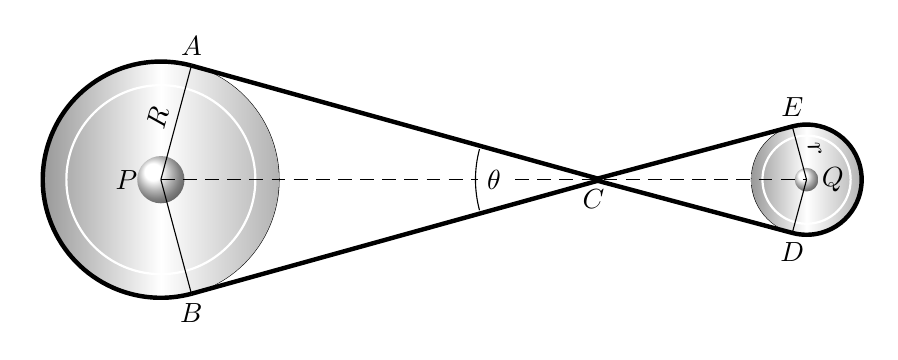
\begin{tikzpicture}
              % Definitions
              \pgfmathsetmacro{\b}{75}
              \pgfmathsetmacro{\a}{15}
              \pgfmathsetmacro{\R}{1.5}
              \pgfmathsetmacro{\r}{0.7}
              \pgfmathsetmacro{\P}{\R*tan(\b)}
              \pgfmathsetmacro{\Q}{\R/cos(\b)}
              \pgfmathsetmacro{\p}{\r/tan(\a)}
              \pgfmathsetmacro{\q}{\r/sin(\a)}

              % Pulleys
              
              % big pulley
              \draw (0,0) circle (\R) ;
              \fill[left color=gray!80, right color=gray!60, middle
                color=white] (0,0) circle (\R) ;
              \draw[thick, white] (0,0) circle (.8*\R);
              \shade[ball color=white] (0,0) circle (.3) node[left,xshift=-5] {$P$};

              % small pulley
              \draw (\Q+\q-.3, 0) circle (\r);
              \fill[left color=gray!80, right color=gray!60, middle
                color=white] (\Q+\q-.3, 0) circle (\r) ;
              \draw[thick, white] (\Q+\q-.3,0) circle (.8*\r);
              \shade[ball color=white] (\Q+\q-.3,0) circle (.15) 
              node[right, xshift=2] {$Q$};

              % belt and point labels
              \begin{scope}[ultra thick]
                \draw (\b:\R) arc (\b:360-\b:\R) ;
                \draw (\b:\R) -- ( \P, 0 ); 
                \draw (-\b:\R) -- ( \P, 0 );
                \draw (\Q-.3,0) -- + (\a:\p)  arc (105:-105:\r) ;
                \draw (\Q-.3,0) -- + (-\a:\p);
                %\draw (\b:\R) arc (\b:360-\b:\r) ;
              \end{scope}
           
              \draw (0,0) -- (\b:\R) node[midway, above,sloped] {$R$} node[above] {$A$};
              \draw (-\b:\R)--(0,0) ;
              \draw (\Q+\q-.3,0) -- +(105:\r) node[midway,above, sloped] {$r$}
                node[above] {$E$};
              \draw (\Q+\q-.3,0) -- +(-105:\r) node[below] {$D$};
              \node[below] at (-\b:\R) {$B$};
              \node[below] at (\Q-.3,0) {$C$};

              % center line
              \draw[dash pattern=on5pt off3pt] (0,0) -- (\Q+\q-.3,0);

              % angle label
              \node[fill=white] at (0.73*\Q, 0) {$\theta$} ;
              \draw (\Q-1.8,0) arc (180:195:1.5);
              \draw (\Q-1.8,0) arc (180:165:1.5);
        \end{tikzpicture}
    \end{center}
    \caption{This is a figure (it uses Ti\emph{k}Z).}
    \label{fig:demo}
\end{figure}
If I put enough text in here then it will be a good example.
Lorem ipsum dolor sit amet, consectetur adipiscing elit.
Maecenas sed est non ipsum egestas scelerisque.
Quisque accumsan eleifend imperdiet.
Quisque odio quam, elementum et interdum eget, ultrices ornare tortor.
Donec sit amet suscipit ligula.
Maecenas neque diam, lobortis ut adipiscing ac, egestas sit amet metus.
Phasellus eu lectus massa, non elementum nunc.
Donec tempor rhoncus condimentum.
Praesent id arcu tortor.

Vivamus ultricies rhoncus risus, ut vehicula dolor hendrerit sit amet.
Fusce dui dolor, feugiat in placerat et, auctor pharetra nibh.
Integer quis mi nulla, quis accumsan est.
Aenean nec mi purus, ut iaculis magna.
Curabitur metus diam, commodo vel feugiat quis, tempor a enim.
Nulla consectetur lorem id arcu ultricies adipiscing.
Donec hendrerit porta feugiat.
Sed eleifend ornare tristique.
Nulla facilisi.
Sed dignissim, libero posuere auctor volutpat, felis quam molestie tortor, eget rutrum nulla est nec leo.
Cras facilisis tortor a nulla semper sed lacinia ligula interdum.
Pellentesque ultrices augue metus.
Vestibulum consectetur quam ac neque venenatis eu tincidunt dui rhoncus.
Mauris ullamcorper enim ac turpis feugiat placerat.
Duis a lorem eget augue malesuada pharetra ut ac felis.

\subsection*{Tables}

A table was already shown, but this one will be at the bottom.
Note the border (I make it manually\dots is there a better way?).
\begin{table}[b]
    \centering
    \caption{A (much) shorter table.}
    \begin{tabular}{|c|c|}
        \hline
        R0C1 & R0C2 \\
        \hline \hline
        R1C1 & R1C2 \\
        R2C1 & R2C2 \\
        \hline
    \end{tabular}
    \label{tab:short}
\end{table}


\section*{Fonts, etc.}

Headings are cap, bold.
No headings are numbered.
Not sure the best way to do this.
Currently I have to star my commands like \verb|\section*{Section}|.
Do you have a better suggestion?

\subsection*{Second-level are bold, title case}

I'm under a second.

\subsubsection*{Third-level are caps, not bold}

I'm under a third.

\section*{Equations}

\dots are why I use \LaTeX .
They are formatted as ASC requires as I can tell.
\begin{equation}
    y(x) = m \cdot x + b
\end{equation}

\section*{The Bibliography}

I'll use the examples straight from the author guide.
We have an article \cite{ikegami1990}, a book \cite{mitsiti1996}, a chapter in a book \cite{inman1998}, a report \cite{margarit1993}, and a presentation at a conference \cite{hoffer1996}.
The numbers in the bibliography are not formatted the same as the author guide, but the entries themselves are at least the correct font size.

\bibliographystyle{asc}
\bibliography{asc-sample}

\end{document}
